% Harus dimuat terlebih dahulu, digunakan agar file PDF memiliki format karakter yang benar.
% Untuk informasi lebih lanjut, lihat https://ctan.org/pkg/cmap.
\RequirePackage{cmap}

% Format dokumen sebagai paper konferensi menggunakan aturan IEEEtran terbaru (v1.8b).
% Untuk informasi lebih lanjut, lihat http://www.michaelshell.org/tex/ieeetran/.
\documentclass[conference]{IEEEtran}[2015/08/26]

% Format encoding font dan input menjadi 8-bit UTF-8.
\usepackage[T1]{fontenc}
\usepackage[utf8]{inputenc}

% Format bahasa menjadi bahasa german dan inggris.
\usepackage[indonesian]{babel}

% Digunakan untuk tujuan demonstrasi.
\usepackage{mwe}

% Digunakan untuk menampilkan font dengan style yang lebih baik.
\usepackage[zerostyle=b,scaled=.75]{newtxtt}

% Digunakan untuk menampilkan tabel dengan style yang lebih baik.
\usepackage{booktabs}

\usepackage{longtable}

% Digunakan untuk menampilkan gambar pada dokumen.
\usepackage{graphicx}

% Digunakan untuk menampilkan potongan kode.
\usepackage{listings}
\lstset{
  basicstyle=\ttfamily,
  columns=fixed,
  basewidth=.5em,
  xleftmargin=0.5cm,
  captionpos=b
}

% Digunakan agar backticks (`) dapat dirender pada PDF.
% Untuk informasi lebih lanjut, lihat https://tex.stackexchange.com/a/341057/9075.
\usepackage{upquote}

% Digunakan untuk menyeimbangkan bagian akhir dokumen dengan dua kolom.
\usepackage{balance}

% Digunakan untuk menampilkan pustaka.
\usepackage[square,comma,numbers,sort&compress]{natbib}

% Mengubah format ukuran teks pada natbib.
\renewcommand{\bibfont}{\normalfont\footnotesize}

% Menambah nama penulis ketika menggunakan perintah \citet.
% Untuk informasi lebih lanjut, lihat https://tex.stackexchange.com/a/76075/9075.
\usepackage{etoolbox}
\makeatletter
\patchcmd{\NAT@test}{\else \NAT@nm}{\else \NAT@hyper@{\NAT@nm}}{}{}
\makeatother

% Digunakan untuk melakukan linewrap pada pustaka dengan url yang panjang
% jika terdapat hyphens
\usepackage[hyphens]{url}

% Digunakan untuk menambah hyperlink pada referensi.
\usepackage{hyperref}

% Menonaktifkan warna dan bookmark pada hyperref.
\hypersetup{hidelinks,
  colorlinks=true,
  allcolors=black,
  pdfstartview=Fit,
  breaklinks=true
}

% Digunakan untuk membenarkan hyperref pada gambar.
\usepackage[all]{hypcap}

% Digunakan untuk menampilkan beberapa gambar
\usepackage[caption=false,font=footnotesize]{subfig}

\usepackage{stfloats}

% Tambahkan format tanda hubung yang benar di sini
\hyphenation{
  ro-ket
  me-ngem-bang-kan
  per-hi-tu-ngan
}

\begin{document}

  % Ubah kalimat berikut sesuai dengan judul penelitian.
\title{Perancangan Sistem Kontrol Motor Kursi Roda Secara Nirkabel Berbasis ESP32}

% Ubah kalimat-kalimat berikut sesuai dengan nama, institusi, alamat dan kontak penulis.
\author{
  \IEEEauthorblockN{I Putu Haris Setiadi Ekatama}
  \IEEEauthorblockA{Departemen Teknik Komputer\\
    Fakultas Teknologi Elektro dan Informatika Cerdas\\
    Institut Teknologi Sepuluh Nopember\\
    Surabaya, Indonesia 60111\\
    \href{mailto:haris.ekatama@gmail.com}{haris.ekatama@gmail.com}}

  \and
  \IEEEauthorblockN{Dr. Eko Mulyanto Yuniarno, S.T., M.T.}
  \IEEEauthorblockA{Departemen Teknik Komputer\\
    Fakultas Teknologi Elektro dan Informatika Cerdas\\
    Institut Teknologi Sepuluh Nopember\\
    Surabaya, Indonesia 60111\\
    \href{mailto:ekomulyanto@ee.its.ac.id}{ekomulyanto@ee.its.ac.id}}
}

% Digunakan untuk menampilkan judul dan deskripsi penulis.
\maketitle

  % Mengubah keterangan `Abstract` ke bahasa indonesia.
% Hapus bagian ini untuk mengembalikan ke format awal.
\renewcommand\abstractname{Abstract}

\begin{abstract}

  % Ubah paragraf berikut sesuai dengan abstrak dari penelitian.
  \emph{Paralysis is a condition where a person experiences a weakening of the functions in their body parts, causing them to lack energy or be unable to move their limbs as they should. There are several conditions that can lead to paralysis, ranging from diseases such as stroke to accidents. Individuals experiencing paralysis often face challenges in their daily mobility. They require additional tools to be able to carry out activities, one of which is a wheelchair. Electric wheelchairs controlled by a joystick have been developed to date. However, the use of a joystick may not address the issues faced by someone experiencing paralysis. This is because individuals with paralysis in their arms may struggle to control this type of electric wheelchair. In this research, a controller for an electric wheelchair has been developed that can be operated through computer vision technology, either with hand poses or head gestures. The integration of this technology can be an innovative solution to the problems being faced. Choosing ESP32 as the main microcontroller is a strategic step due to its ability to precisely control the wheelchair's motor. In addition to functioning as a motor controller, ESP32 also serves as a data receiver from the computer equipped with computer vision technology. From the test results, it is concluded that the transmission from computer vision should be analogized to 1 character letter and transmitted using WiFi. This is done because transmitting data containing 1 letter and using WiFi has the best delay time, which is 0.03499708571 seconds. Through this integration, it is expected that the motor controller can operate synergistically with the information received from the computer, creating an efficient and responsive system.}

\end{abstract}

% Mengubah keterangan `Index terms` ke bahasa indonesia.
% Hapus bagian ini untuk mengembalikan ke format awal.
\renewcommand\IEEEkeywordsname{Keywords}

\begin{IEEEkeywords}

  % Ubah kata-kata berikut sesuai dengan kata kunci dari penelitian.
  \emph{Wheelchair}, \emph{Convolutional Neural Network}, \emph{Mediapipe}, \emph{ESP32}, \emph{WiFi}.

\end{IEEEkeywords}


  % Ubah bagian berikut sesuai dengan konten-konten yang akan dimasukkan pada dokumen
  % Ubah judul dan label berikut sesuai dengan yang diinginkan.
\section{Pendahuluan}
\label{sec:pendahuluan}

% Ubah paragraf-paragraf pada bagian ini sesuai dengan yang diinginkan.

Menurut Kamus Besar Bahasa Indonesia, lumpuh merupakan melemahnya fungsi anggota badan sehingga tidak bertenaga atau tidak dapat digerakkan lagi sebagaimana mestinya \cite{Daring_2016}. Otot beserta tulang, saraf, serta jaringan penghubung antara otot, tulang dan saraf memiliki peran yang penting dalam mengendalikan gerak tubuh manusia. Apabila salah satu jaringan mengalami gangguan makan akan terjadi kelumpulan, baik kelumpuhan sementara maupun kelumpuhan permanen.

Terdapat beberapa kondisi yang dapat mengakibatkan kelumpuhan, seperti penyakit stroke yang dapat menyebabkan kelumpuhan pada salah satu sisi wajah, lengan serta tungkai, \emph{Bell's Palsy} yang dapat menyebabkan kelumpuhan pada salah satu sisi wajah tanpa disertai kelumpuhan pada anggota tubuh yang lain, cedera otak yang dapat memicu kelumpuhan pada setiap bagian tubuh sesuai bagian otak yang rusak, polio yang menyebabkan kelumpuhan pada lengan, tungkai, serta otot pernapasan, dan masih banyak kondisi yang menyebabkan kelumpuhan \cite{Pansawira_2022}.

Seseorang yang mengalami kelumpuhan sering kali mengalami permasalahan dalam hal mobilitas sehari-hari. Mereka memerlukan alat tambahan untuk dapat beraktivitas sehari-hari, salah satunya adalah kursi roda. Hingga saat ini sudah terdapat kursi roda elektrik yang dikendalikan dengan menggunakan \emph{joystick} \cite{choi2019motion}. Akan tetapi penggunaan \emph{joystick} belum dapat menjawab permasalahan dari seseorang yang mengalami kelumpuhan. Karena bagi orang yang mengalami kelumpuhan pada bagian lengan akan kekusahan dalam mengendalikan kursi roda elektrik berjenis ini.

Dalam menghadapi permasalahan kelumpuhan, sangat penting untuk mencari solusi yang dapat meningkatkan kemandirian para penderita. Salah satu pendekatan yang menjanjikan adalah memanfaatkan teknologi canggih, seperti visi komputer yang dapat diintegrasikan dengan sistem tertanam. Dengan menggabungkan kedua teknologi ini, diharapkan dapat diciptakan solusi inovatif yang memungkinkan para penderita kelumpuhan untuk tetap dapat bermobilitas secara mandiri.

Visi komputer merupakan bidang keilmuan yang memungkinkan komputer dapat "melihat" \cite{TIAN20201}. Teknologi ini menggunakan kamera untuk mengidentifikasi, melacak, hingga mengukur target untuk pemrosesan citra lebih lanjut. Visi komputer memberikan kemampuan untuk mengenali dan memahami lingkungan sekitar. Sedangkan sistem tertanam dapat diatur secara personal untuk memenuhi kebutuhan spesifik sesuai dengan permasalahan yang dihadapi. 

Integrasi teknologi ini dapat menjadi solusi inovatif terhadap permasalahan yang dihadapi. Dalam rangka mengatasi tantangan ini, penelitian akan difokuskan pada pengembangan kontroler motor yang dapat secara optimal berinteraksi dengan teknologi visi komputer. Pemilihan ESP32 sebagai mikrokontroler utama menjadi langkah strategis, karena kemampuannya dalam mengatur dengan presisi kerja motor. Tidak hanya berfungsi sebagai kontroler motor, ESP32 juga akan berperan sebagai perangkat penerima data dari komputer yang dilengkapi dengan teknologi visi komputer. Melalui integrasi ini, diharapkan bahwa kontroler motor dapat beroperasi secara sinergis dengan informasi yang diterima dari komputer dan menciptakan sebuah sistem yang efisien dan responsif. 

  % Ubah judul dan label berikut sesuai dengan yang diinginkan.
\section{Methodology}
\label{sec:metodologi}

% Ubah paragraf-paragraf pada bagian ini sesuai dengan yang diinginkan.
This research is conducted in accordance with the following system design along with its implementation. The system design is the concept of creating and designing infrastructure, which is then manifested in the form of flow blocks that need to be executed.

In this research, a device integrated with computer vision technology will be developed to control the movement of a wheelchair. Generally, this study will employ a system design as depicted in Figure \ref{fig:Metodologi Penelitian}.

% Gambar 3.1
\begin{figure} [ht] \centering
    % Nama dari file gambar yang diinputkan
    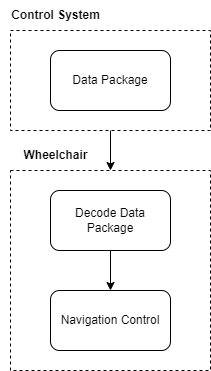
\includegraphics[scale=0.8]{gambar/block diagram.png}
    % Keterangan gambar yang diinputkan
    \caption{Research Block Diagram}
    % Label referensi dari gambar yang diinputkan
    \label{fig:Metodologi Penelitian}
\end{figure}

\subsection{Data Package}
To move the wheelchair, commands need to be sent to the wheelchair controller. In the pose classification phase, basic commands for moving the wheelchair have been obtained, such as forward, backward, right, left, and stop. These commands will then be combined with the maximum speed to form a command or data packet like "Direction, Speed". Direction is a variable with the data type "char" used to control the direction of the wheelchair motor movement. Speed is a variable with the data type "char" used to control the maximum speed of the wheelchair motor rotation.

The direction variable has a "char" data type that determines the movement of the wheelchair motor, while the speed variable has a "char" data type that determines the maximum speed of the wheelchair. To reduce data size, the instruction code to determine the movement direction and maximum speed will be represented by a single letter. The instruction codes can be seen in Table \ref{tbl:kode-instruksi} and Table \ref{tbl:kodePWM}.

After these two variables are combined, they will be sent wirelessly, either using Bluetooth or WiFi, from the laptop or Jetson Nano to the ESP32.
% Tabel 3.2
\begin{table}[h]
  \centering
      \caption{The instruction codes from the pose classification results}
      \label{tbl:kode-instruksi}
      \begin{tabular}{|c|c|}
          \hline
          Pose Classification & Instruction Code \\ \hline
          Left             & A              \\ \hline
          Forward             & B              \\ \hline
          Stop             & C              \\ \hline
          Reverse           & D              \\ \hline
          Right            & E              \\ \hline
      \end{tabular}
\end{table}

\begin{table}[!ht]
    \centering
    \caption{The instruction code for controlling the PWM level}
    \label{tbl:kodePWM}
    \begin{tabular}{|c|c|}
    \hline
    Maximum PWM & Instruction Code \\ \hline
    0           & O                \\ \hline
    31          & P                \\ \hline
    63          & Q                \\ \hline
    95          & R                \\ \hline
    127         & S                \\ \hline
    159         & T                \\ \hline
    191         & U                \\ \hline
    223         & V                \\ \hline
    255         & W                \\ \hline
    \end{tabular}
    \end{table}

After combining both variables, they will be wirelessly transmitted, either using Bluetooth or WiFi, from a laptop or Jetson Nano to the ESP32.

\subsection{Decode Data Package}
The data package sent through the laptop or Jetson Nano will be received by the ESP32 using Bluetooth or WiFi. Upon reception by the ESP32, the data undergoes a series of processes involving data package decoding and adjustment according to the predefined variables. This decoding process allows the ESP32 to decompose the information contained in each package and ensure that each variable is accurately separated. Thus, this process organizes and rearranges the information, ensuring that each variable aligns correctly with the provided variable names and data types.

\subsection{Navigation Control}
Both variables obtained from decoding the data package will be processed on the ESP32. The direction variable will play a role in determining the motor's movement direction, while the speed variable will be used to set the maximum speed of the motor movement. There is a series of chained 'if' logics in the navigation control, where the four direction variables will determine the motor rotation direction. Additionally, the maximum PWM value is configured using the speed variable, allowing users to adjust the maximum motor speed as desired. Thus, at this stage, the ESP32 can effectively process the data received through the wireless system and generate corresponding control instructions to move the wheelchair in the desired direction and speed.
  % Ubah judul dan label berikut sesuai dengan yang diinginkan.
\section{Architecture}
\label{sec:arsitektur}

% Ubah paragraf-paragraf pada bagian ini sesuai dengan yang diinginkan.
In this study, a control device has been developed that can receive commands wirelessly from other devices such as a laptop or Jetson Nano. This subsection will detail the implementation of the device developed in this research.

Below are detailed some of the hardware and software used in this research, as follows:
\begin{enumerate}
    \item Anaconda Navigator
    \item Arduino IDE 
    \item Laptop 
    \item Jetson Nano
    \item Camera
    \item ESP32 Devkit V1
    \item 2 Motor Driver
    \item 2 DC-DC Voltage Regulator
    \item 2 DC Motor
    \item 24V Battery
\end{enumerate}

\subsection{Schematic}
\label{subsec:skematik alat}

The schematic of this device is illustrated in detail in Figure \ref{fig:Skematik Alat}. This system utilizes a camera connected to a laptop or Jetson Nano as the main device for capturing images. The workflow begins when the camera captures images of the object. These captured images are then processed by the laptop or Jetson Nano. In this system, a pre-programmed classification model plays a crucial role in interpreting the image data. The results of this classification process are crucial as they form the basis for determining the instruction codes to be implemented.

The instruction codes will then be combined with the maximum speed parameters previously set by the user. The combination of instruction codes and speed parameters will form a data package as wheelchair motion control. This data package will then be transmitted wirelessly, either via Bluetooth or WiFi, to the ESP32 Devkit V1 module.

The ESP32 plays a crucial role in controlling the wheelchair motor. The ESP32 will serve as the control center that receives the data package sent wirelessly by the user. Subsequently, the ESP32 will decode the data package and adjust the data into predefined variables. This data package decoding process will yield two main pieces of data, which will then be further processed by the ESP32.

The first variable is the direction variable, which plays a crucial role in determining the direction of movement for the wheelchair's two motors. This variable ensures that the motors move in the desired direction based on the received data. Additionally, there is the speed variable used to set the maximum speed of the motor movement.

In its implementation, there is a series of chained 'if' logics that will be detailed in the programming subsection. Simply put, this chained 'if' logic plays a crucial role in decision-making for both the direction and speed of the motors based on the received data. The result of this logic will provide triggers in the form of either 5V or 0V. This voltage will then influence the motor rotation direction.

Next, the speed variable will be used to adjust the Pulse Width Modulation (PWM) level on the motor controller. This PWM adjustment is crucial for controlling the motor rotation speed. By adjusting the PWM level, the maximum motor speed can be customized according to the requirements.

\begin{figure} [!ht] \centering
  % Nama dari file gambar yang diinputkan
  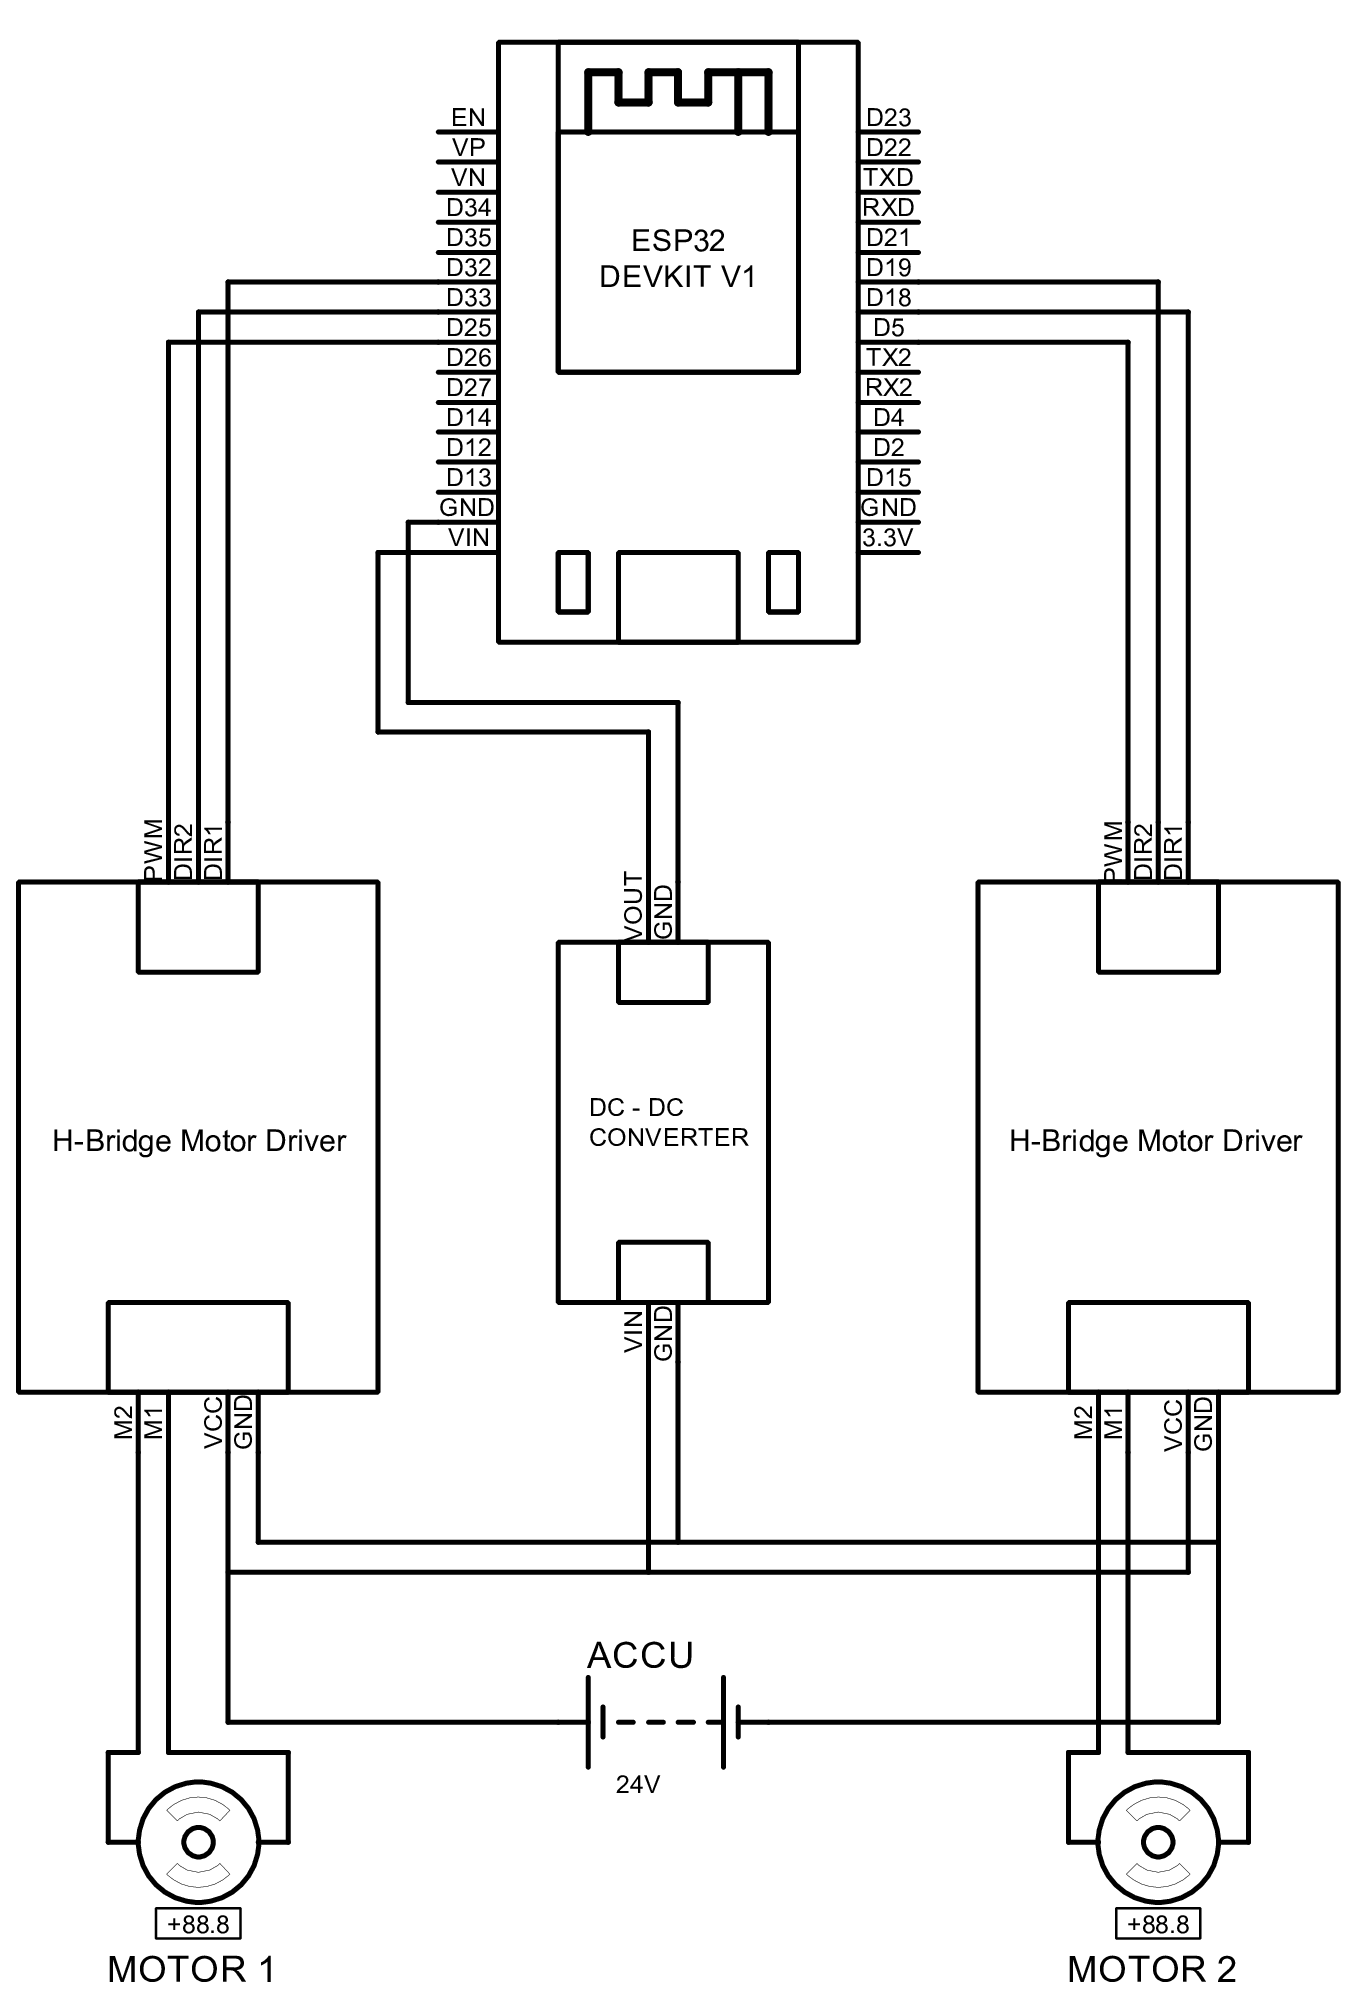
\includegraphics[scale=0.24]{gambar/bab3/Schematics.png}
  % Keterangan gambar yang diinputkan
  \caption{Schematic of the wheelchair motor control}
  % Label referensi dari gambar yang diinputkan
  \label{fig:Skematik Alat}
\end{figure}


  % Ubah judul dan label berikut sesuai dengan yang diinginkan.
\section{Testing Results}
\label{sec:hasil pengujian}

% Ubah paragraf-paragraf pada bagian ini sesuai dengan yang diinginkan.
In this chapter, several testing scenarios, as outlined in the methodology, will be discussed. These scenarios are designed to determine the delay time required to transmit data from the laptop to the ESP32. The testing scenarios to be implemented will cover the following points:

\begin{enumerate}
  \item Testing the delay time for String data transmission via Bluetooth
  \item Testing the delay time for JSON data transmission via Bluetooth
  \item Testing the delay time for String data transmission via WiFi Access Point
  \item Testing the delay time for JSON data transmission via WiFi Access Point
\end{enumerate}

The implementation of the methodology and testing scenarios that will be presented in this chapter is expected to provide an understanding of the results and discussions, allowing conclusions to be drawn from the completed Final Project.

\subsection{Testing The Delay Time for String Data Transmission via Bluetooth}

The testing of data transmission delay is conducted by sending string data from a laptop to ESP32 via Bluetooth. The transmitted data includes direction and speed, separated by a comma as depicted in Equation \ref{eq:string-2data}.

\begin{equation}
  \label{eq:string-2data}
    Direction(char),Speed(integer)
\end{equation}

The direction variable has a data type of `char` used to determine the movement direction of the wheelchair motor, while the speed variable has an integer data type that will specify the maximum speed of the wheelchair motor rotation. The results of the testing for the delay time of string data transmission via Bluetooth can be seen in Table \ref{tbl:delayBluetooth} and Table \ref{tbl:delayBluetooth1}.

\begin{table}[!ht]
\centering
  \caption{Testing the Delay Time of String Data Transmission Containing 2 Values Via Bluetooth}
  \label{tbl:delayBluetooth}
  \begin{tabular}{|ccc|c|}
  \hline
  \multicolumn{1}{|c|}{Data}  & \multicolumn{1}{c|}{Timestamp Send}  & Timestamp Received & Delay Time  \\ \hline
  \multicolumn{1}{|c|}{C,40}  & \multicolumn{1}{c|}{22:02:06.857715} & 22:02:07.892       & 1,034285    \\ \hline
  \multicolumn{1}{|c|}{A,226} & \multicolumn{1}{c|}{22:02:08.358496} & 22:02:09.390       & 1,031504    \\ \hline
  \multicolumn{1}{|c|}{E,21}  & \multicolumn{1}{c|}{22:02:09.859346} & 22:02:10.921       & 1,061654    \\ \hline
  \multicolumn{1}{|c|}{C,168} & \multicolumn{1}{c|}{22:02:11.360115} & 22:02:12.405       & 1,044885    \\ \hline
  \multicolumn{1}{|c|}{B,247} & \multicolumn{1}{c|}{22:02:12.860932} & 22:02:13.900       & 1,039068    \\ \hline
  \multicolumn{1}{|c|}{B,72}  & \multicolumn{1}{c|}{22:02:14.361692} & 22:02:15.400       & 1,038308    \\ \hline
  \multicolumn{1}{|c|}{E,129} & \multicolumn{1}{c|}{22:05:28.232092} & 22:05:29.283       & 1,050908    \\ \hline
  \multicolumn{1}{|c|}{D,117} & \multicolumn{1}{c|}{22:05:29.732554} & 22:05:30.765       & 1,032446    \\ \hline
  \multicolumn{1}{|c|}{C,31}  & \multicolumn{1}{c|}{22:05:31.233293} & 22:05:32.264       & 1,030707    \\ \hline
  \multicolumn{1}{|c|}{B,248} & \multicolumn{1}{c|}{22:05:32.734151} & 22:05:33.779       & 1,044849    \\ \hline
  \multicolumn{1}{|c|}{D,126} & \multicolumn{1}{c|}{22:05:34.235059} & 22:05:35.271       & 1,035941    \\ \hline
  \multicolumn{1}{|c|}{C,2}   & \multicolumn{1}{c|}{22:07:30.543505} & 22:07:31.599       & 1,055495    \\ \hline
  \multicolumn{1}{|c|}{B,29}  & \multicolumn{1}{c|}{22:07:32.044303} & 22:07:33.077       & 1,032697    \\ \hline
  \multicolumn{1}{|c|}{C,247} & \multicolumn{1}{c|}{22:07:33.545370} & 22:07:34.595       & 1,04963     \\ \hline
  \multicolumn{1}{|c|}{A,190} & \multicolumn{1}{c|}{22:07:35.046573} & 22:07:36.085       & 1,038427    \\ \hline
  \multicolumn{1}{|c|}{A,49}  & \multicolumn{1}{c|}{22:07:36.547315} & 22:07:37.575       & 1,027685    \\ \hline
  \multicolumn{1}{|c|}{B,25}  & \multicolumn{1}{c|}{22:09:44.370413} & 22:09:45.405       & 1,034587    \\ \hline
  \multicolumn{1}{|c|}{D,72}  & \multicolumn{1}{c|}{22:09:45.871428} & 22:09:46.921       & 1,049572    \\ \hline
  \multicolumn{1}{|c|}{C,63}  & \multicolumn{1}{c|}{22:09:47.372407} & 22:09:48.415       & 1,042593    \\ \hline
  \multicolumn{1}{|c|}{A,245} & \multicolumn{1}{c|}{22:09:48.873310} & 22:09:49.885       & 1,01169     \\ \hline
  \multicolumn{1}{|c|}{C,70}  & \multicolumn{1}{c|}{22:09:50.374135} & 22:09:51.406       & 1,031865    \\ \hline
  \multicolumn{1}{|c|}{D,240} & \multicolumn{1}{c|}{22:09:51.874944} & 22:09:52.929       & 1,054056    \\ \hline
  \multicolumn{1}{|c|}{A,46}  & \multicolumn{1}{c|}{22:11:46.717729} & 22:11:47.744       & 1,026271    \\ \hline
  \multicolumn{1}{|c|}{B,245} & \multicolumn{1}{c|}{22:11:48.218593} & 22:11:49.263       & 1,044407    \\ \hline
  \multicolumn{1}{|c|}{B,68}  & \multicolumn{1}{c|}{22:11:49.719513} & 22:11:50.763       & 1,043487    \\ \hline
  \multicolumn{1}{|c|}{E,204} & \multicolumn{1}{c|}{22:11:51.219962} & 22:11:52.271       & 1,051038    \\ \hline
  \multicolumn{1}{|c|}{B,26}  & \multicolumn{1}{c|}{22:11:52.720738} & 22:11:53.746       & 1,025262    \\ \hline
  \multicolumn{1}{|c|}{D,113} & \multicolumn{1}{c|}{22:13:39.843434} & 22:13:40.871       & 1,027566    \\ \hline
  \multicolumn{1}{|c|}{B,195} & \multicolumn{1}{c|}{22:13:41.344420} & 22:13:42.389       & 1,04458     \\ \hline
  \multicolumn{1}{|c|}{A,242} & \multicolumn{1}{c|}{22:13:42.845419} & 22:13:43.876       & 1,030581    \\ \hline
  \multicolumn{1}{|c|}{A,17}  & \multicolumn{1}{c|}{22:13:44.346312} & 22:13:45.360       & 1,013688    \\ \hline
  \multicolumn{1}{|c|}{A,140} & \multicolumn{1}{c|}{22:13:45.847280} & 22:13:46.915       & 1,06772     \\ \hline
  \multicolumn{3}{|c|}{Average Delay Time}                                                & 1,038982875 \\ \hline
  \end{tabular}
\end{table}

Table \ref{tbl:delayBluetooth} displays the transmission of string data consisting of 2 values separated by a comma (","). In this test, data is sent 32 times consecutively with an added delay time of 1.5 seconds each time data is transmitted. This is done to ensure that the ESP32 can receive the data properly and successfully separate and insert the two values according to the predefined variables. The results of this test indicate that the average transmission time from the laptop to the ESP32 via Bluetooth is 1.038982875 seconds.

\begin{table}[!h]
\centering
  \caption{Testing the Delay Time of String Data Transmission Containing 1 Value Via Bluetooth}
  \label{tbl:delayBluetooth1}
  \begin{tabular}{|ccc|c|}
  \hline
  \multicolumn{1}{|c|}{Data} & \multicolumn{1}{c|}{Timestamp Sent}  & Timestamp Received & Delay Time   \\ \hline
  \multicolumn{1}{|c|}{D}    & \multicolumn{1}{c|}{17:56:13.163165} & 17:56:14.352       & 1,189        \\ \hline
  \multicolumn{1}{|c|}{E}    & \multicolumn{1}{c|}{17:56:14.260985} & 17:56:14.491       & 0,230        \\ \hline
  \multicolumn{1}{|c|}{D}    & \multicolumn{1}{c|}{17:56:14.442510} & 17:56:14.708       & 0,265        \\ \hline
  \multicolumn{1}{|c|}{E}    & \multicolumn{1}{c|}{17:56:14.649861} & 17:56:14.878       & 0,228        \\ \hline
  \multicolumn{1}{|c|}{D}    & \multicolumn{1}{c|}{17:56:14.782992} & 17:56:15.017       & 0,234        \\ \hline
  \multicolumn{1}{|c|}{C}    & \multicolumn{1}{c|}{17:56:14.957997} & 17:56:15.188       & 0,230        \\ \hline
  \multicolumn{1}{|c|}{A}    & \multicolumn{1}{c|}{17:56:15.096377} & 17:56:15.311       & 0,215        \\ \hline
  \multicolumn{1}{|c|}{D}    & \multicolumn{1}{c|}{17:56:15.255594} & 17:56:15.483       & 0,227        \\ \hline
  \multicolumn{1}{|c|}{D}    & \multicolumn{1}{c|}{17:56:15.406847} & 17:56:15.745       & 0,338        \\ \hline
  \multicolumn{1}{|c|}{E}    & \multicolumn{1}{c|}{17:56:15.663510} & 17:56:15.930       & 0,266        \\ \hline
  \multicolumn{1}{|c|}{D}    & \multicolumn{1}{c|}{17:56:15.893686} & 17:56:16.195       & 0,301        \\ \hline
  \multicolumn{1}{|c|}{C}    & \multicolumn{1}{c|}{17:56:16.118896} & 17:56:16.320       & 0,201        \\ \hline
  \multicolumn{1}{|c|}{A}    & \multicolumn{1}{c|}{17:56:16.287623} & 17:56:16.458       & 0,170        \\ \hline
  \multicolumn{1}{|c|}{A}    & \multicolumn{1}{c|}{17:56:16.416326} & 17:56:16.674       & 0,258        \\ \hline
  \multicolumn{1}{|c|}{A}    & \multicolumn{1}{c|}{17:56:16.600528} & 17:56:16.862       & 0,261        \\ \hline
  \multicolumn{1}{|c|}{C}    & \multicolumn{1}{c|}{17:56:16.800782} & 17:56:17.080       & 0,279        \\ \hline
  \multicolumn{1}{|c|}{A}    & \multicolumn{1}{c|}{17:56:16.972893} & 17:56:17.360       & 0,387        \\ \hline
  \multicolumn{1}{|c|}{C}    & \multicolumn{1}{c|}{17:56:17.250136} & 17:56:17.641       & 0,391        \\ \hline
  \multicolumn{1}{|c|}{B}    & \multicolumn{1}{c|}{17:56:17.544344} & 17:56:17.779       & 0,235        \\ \hline
  \multicolumn{1}{|c|}{C}    & \multicolumn{1}{c|}{17:56:17.728154} & 17:56:18.012       & 0,284        \\ \hline
  \multicolumn{1}{|c|}{A}    & \multicolumn{1}{c|}{17:56:17.945683} & 17:56:18.151       & 0,205        \\ \hline
  \multicolumn{1}{|c|}{D}    & \multicolumn{1}{c|}{17:56:18.097472} & 17:56:18.382       & 0,285        \\ \hline
  \multicolumn{1}{|c|}{A}    & \multicolumn{1}{c|}{17:56:18.302853} & 17:56:18.614       & 0,311        \\ \hline
  \multicolumn{1}{|c|}{D}    & \multicolumn{1}{c|}{17:56:18.550624} & 17:56:18.818       & 0,267        \\ \hline
  \multicolumn{1}{|c|}{B}    & \multicolumn{1}{c|}{17:56:18.745921} & 17:56:18.990       & 0,244        \\ \hline
  \multicolumn{1}{|c|}{A}    & \multicolumn{1}{c|}{17:56:18.932188} & 17:56:19.162       & 0,230        \\ \hline
  \multicolumn{1}{|c|}{B}    & \multicolumn{1}{c|}{17:56:19.129604} & 17:56:19.596       & 0,466        \\ \hline
  \multicolumn{1}{|c|}{C}    & \multicolumn{1}{c|}{17:56:19.482713} & 17:56:19.937       & 0,454        \\ \hline
  \multicolumn{1}{|c|}{C}    & \multicolumn{1}{c|}{17:56:19.876232} & 17:56:20.341       & 0,465        \\ \hline
  \multicolumn{1}{|c|}{C}    & \multicolumn{1}{c|}{17:56:20.216948} & 17:56:20.649       & 0,432        \\ \hline
  \multicolumn{1}{|c|}{E}    & \multicolumn{1}{c|}{17:56:20.588913} & 17:56:21.052       & 0,463        \\ \hline
  \multicolumn{1}{|c|}{B}    & \multicolumn{1}{c|}{17:56:20.913091} & 17:56:21.468       & 0,555        \\ \hline
  \multicolumn{1}{|c|}{C}    & \multicolumn{1}{c|}{17:56:21.323255} & 17:56:21.873       & 0,550        \\ \hline
  \multicolumn{1}{|c|}{C}    & \multicolumn{1}{c|}{17:56:21.820789} & 17:56:22.278       & 0,457        \\ \hline
  \multicolumn{1}{|c|}{B}    & \multicolumn{1}{c|}{17:56:22.149208} & 17:56:22.807       & 0,658        \\ \hline
  \multicolumn{3}{|c|}{Average Delay Time}                                               & 0,3495228571 \\ \hline
  \end{tabular}
\end{table}

Table \ref{tbl:delayBluetooth1} presents the transmission of string data consisting of 1 value, namely direction. In this test, data is sent 35 times consecutively without adding delay time each time data is transmitted. The results of this test indicate that the average transmission time from the laptop to the ESP32 via Bluetooth is 0.3495228571 seconds.

A significant delay time difference was found between the process of sending a string containing 2 values compared to a string with only 1 value. When sending a string containing 2 data, the test indicated a delay time of approximately 1.038982875 seconds. In comparison with the test involving a string with 1 value, the recorded delay time was only about 0.3495228571 seconds. It is important to note that there is a drawback when sending a string containing 2 values, namely the addition of a 1.5-second delay each time data transmission is carried out. This is done to ensure optimal data reception by the ESP32. Therefore, it can be concluded that in the context of data transmission via Bluetooth, it is advisable to send a string with only 1 value to avoid additional delays that may affect the overall efficiency and speed of data transmission.

\subsection{Testing The Delay Time for JSON Data Transmission via Bluetooth}

The testing of data transmission delay is conducted by sending JSON data from a laptop to ESP32 via Bluetooth. The transmitted data includes direction and speed, formatted into JSON as shown in Equation \ref{eq:json-2data}, and also JSON containing only direction data as depicted in Equation \ref{eq:json-1data}.

\begin{equation}
  \label{eq:json-2data}
    \{'arah': Direction(char), 'kecepatan': Speed(integer)\}
\end{equation}

\begin{equation}
  \label{eq:json-1data}
    \{'arah': Direction(char)\}
\end{equation}

The JSON data consists of two parts: the key and the value. There are two keys, namely 'direction' and 'speed.' The 'direction' key contains a char data type value used to determine the direction of the wheelchair motor, while the 'speed' key contains an integer data type value used to set the maximum speed of the wheelchair motor rotation. The results of the JSON data transmission delay test can be seen in Table \ref{tbl:delayBluetoothJSON2} and Table \ref{tbl:delayBluetoothJSON1}.

\begin{table}[!h]
\centering
  \caption{Testing the Delay Time of Sending JSON Data Containing 2 Values Via Bluetooth}
  \label{tbl:delayBluetoothJSON2}
  \begin{tabular}{|c|c|}
  \hline
  Data                              & Delay Time  \\ \hline
  \{'arah': 'C', 'kecepatan': 73\}  & 1,070983    \\ \hline
  \{'arah': 'D', 'kecepatan': 69\}  & 1,043823    \\ \hline
  \{'arah': 'D', 'kecepatan': 140\} & 1,077356    \\ \hline
  \{'arah': 'A', 'kecepatan': 112\} & 1,044772    \\ \hline
  \{'arah': 'B', 'kecepatan': 125\} & 1,032068    \\ \hline
  \{'arah': 'A', 'kecepatan': 141\} & 1,068203    \\ \hline
  \{'arah': 'D', 'kecepatan': 210\} & 1,096744    \\ \hline
  \{'arah': 'E', 'kecepatan': 48\}  & 1,050115    \\ \hline
  \{'arah': 'D', 'kecepatan': 247\} & 1,035611    \\ \hline
  \{'arah': 'E', 'kecepatan': 48\}  & 1,081798    \\ \hline
  \{'arah': 'A', 'kecepatan': 117\} & 1,104833    \\ \hline
  \{'arah': 'B', 'kecepatan': 175\} & 1,042016    \\ \hline
  \{'arah': 'C', 'kecepatan': 121\} & 1,026936    \\ \hline
  \{'arah': 'E', 'kecepatan': 55\}  & 1,070894    \\ \hline
  \{'arah': 'A', 'kecepatan': 134\} & 1,097328    \\ \hline
  \{'arah': 'A', 'kecepatan': 241\} & 1,038598    \\ \hline
  \{'arah': 'C', 'kecepatan': 8\}   & 1,041939    \\ \hline
  \{'arah': 'C', 'kecepatan': 242\} & 1,061519    \\ \hline
  \{'arah': 'E', 'kecepatan': 251\} & 1,098049    \\ \hline
  \{'arah': 'C', 'kecepatan': 65\}  & 1,010486    \\ \hline
  \{'arah': 'B', 'kecepatan': 184\} & 1,044790    \\ \hline
  \{'arah': 'D', 'kecepatan': 244\} & 1,065066    \\ \hline
  \{'arah': 'D', 'kecepatan': 216\} & 1,092696    \\ \hline
  \{'arah': 'E', 'kecepatan': 209\} & 1,048105    \\ \hline
  \{'arah': 'C', 'kecepatan': 131\} & 1,039553    \\ \hline
  \{'arah': 'D', 'kecepatan': 172\} & 1,060164    \\ \hline
  \{'arah': 'C', 'kecepatan': 166\} & 1,062550    \\ \hline
  \{'arah': 'E', 'kecepatan': 47\}  & 1,047506    \\ \hline
  \{'arah': 'E', 'kecepatan': 193\} & 1,052148    \\ \hline
  \{'arah': 'A', 'kecepatan': 54\}  & 1,062337    \\ \hline
  \{'arah': 'B', 'kecepatan': 158\} & 1,066952    \\ \hline
  Average Delay Time                & 1,059223806 \\ \hline
  \end{tabular}
\end{table}

Table \ref{tbl:delayBluetoothJSON2} displays the transmission of JSON containing 2 key-value pairs, namely 'direction' and 'speed.' In this test, the data was sent 31 times consecutively, with an additional delay of 1.1 seconds for each data transmission. This was done to ensure that the ESP32 could receive the data properly and successfully separate (deserialize) and input both values according to the specified variables. The results of this test indicate that the average transmission time from the laptop to the ESP32 via Bluetooth is approximately 1.059223806 seconds.

\begin{table}[!h]
\centering
  \caption{Testing the Delay Time of Sending JSON Data Containing 1 Value Via Bluetooth}
  \label{tbl:delayBluetoothJSON1}
  \begin{tabular}{|c|c|}
  \hline
  Data               & Delay Time  \\ \hline
  \{'arah': 'B'\}    & 1,063216    \\ \hline
  \{'arah': 'D'\}    & 1,050613    \\ \hline
  \{'arah': 'E'\}    & 1,056152    \\ \hline
  \{'arah': 'A'\}    & 1,052444    \\ \hline
  \{'arah': 'C'\}    & 1,039226    \\ \hline
  \{'arah': 'C'\}    & 1,138351    \\ \hline
  \{'arah': 'B'\}    & 1,035915    \\ \hline
  \{'arah': 'D'\}    & 1,056977    \\ \hline
  \{'arah': 'C'\}    & 1,049147    \\ \hline
  \{'arah': 'D'\}    & 1,131767    \\ \hline
  \{'arah': 'C'\}    & 1,137578    \\ \hline
  \{'arah': 'B'\}    & 1,054065    \\ \hline
  \{'arah': 'E'\}    & 1,056702    \\ \hline
  \{'arah': 'E'\}    & 1,052598    \\ \hline
  \{'arah': 'E'\}    & 1,048436    \\ \hline
  \{'arah': 'C'\}    & 1,054793    \\ \hline
  \{'arah': 'A'\}    & 1,059857    \\ \hline
  \{'arah': 'E'\}    & 1,054579    \\ \hline
  \{'arah': 'E'\}    & 1,129237    \\ \hline
  \{'arah': 'E'\}    & 1,031556    \\ \hline
  \{'arah': 'D'\}    & 1,062512    \\ \hline
  \{'arah': 'C'\}    & 1,134129    \\ \hline
  \{'arah': 'D'\}    & 1,11367     \\ \hline
  \{'arah': 'A'\}    & 1,051385    \\ \hline
  \{'arah': 'E'\}    & 1,120536    \\ \hline
  \{'arah': 'B'\}    & 1,116529    \\ \hline
  \{'arah': 'A'\}    & 1,060862    \\ \hline
  \{'arah': 'D'\}    & 1,057455    \\ \hline
  \{'arah': 'C'\}    & 1,060398    \\ \hline
  \{'arah': 'C'\}    & 1,04322     \\ \hline
  \{'arah': 'C'\}    & 1,049035    \\ \hline
  \{'arah': 'C'\}    & 1,101292    \\ \hline
  \{'arah': 'D'\}    & 1,016585    \\ \hline
  \{'arah': 'B'\}    & 1,045899    \\ \hline
  \{'arah': 'D'\}    & 1,044521    \\ \hline
  Average Delay Time & 1,069463914 \\ \hline
  \end{tabular}
\end{table}

Table \ref{tbl:delayBluetoothJSON1} illustrates the transmission of JSON containing 1 key-value pair, namely 'direction.' In this test, the data was sent 35 times consecutively, with an additional delay of 1 second for each data transmission. This was done to ensure that the ESP32 could receive the data properly and successfully separate (deserialize) and input the value according to the specified variable. The results of this test indicate an average transmission time from the laptop to the ESP32 via Bluetooth of approximately 1.069463914 seconds.

Different testing methods revealed that the delay time between the transmission processes of JSON containing 2 key-value pairs and JSON containing only 1 key-value pair is not significantly different. When sending JSON with 2 key-value pairs, the test showed a delay of approximately 1.059223806 seconds. In comparison, the recorded delay time for the test involving JSON with 1 key-value pair was approximately 1.069463914 seconds. An anomaly was observed in this test, as the delay time when sending JSON with 2 key-value pairs was shorter compared to sending JSON with 1 key-value pair, even though the difference in delay time was not significant.

\subsection{Testing The Delay Time for String Data Transmission via WiFi Access Point}

The delay time testing for data transmission was conducted by sending String data from the laptop to the ESP32 via WiFi. The ESP32 was set up as an Access Point. The transmitted data included direction and speed data separated by a comma, as shown in Equation \ref{eq:string-2Data}.

\begin{equation}
  \label{eq:string-2Data}
    Direction(char),Speed(integer)
\end{equation}

The direction variable has a char data type used to determine the direction of the wheelchair motor, while the speed variable has an integer data type that will determine the maximum speed of the wheelchair motor rotation. The results of the delay time testing for String data transmission via WiFi can be seen in Table \ref{tbl:delayWiFi2} and Table \ref{tbl:delayWiFi1}.

\begin{table}[!h]
\centering
  \caption{Testing the delay time of sending String data containing 2 values via WiFi Access Point}
  \label{tbl:delayWiFi2}
  \begin{tabular}{|ccc|c|}
  \hline
  \multicolumn{1}{|c|}{Data}  & \multicolumn{1}{c|}{Timestamp Sent}  & Timestamp Received & Delay Time  \\ \hline
  \multicolumn{1}{|c|}{D,175} & \multicolumn{1}{c|}{22:34:36.127972} & 22:34:37.159       & 1,031028    \\ \hline
  \multicolumn{1}{|c|}{D,220} & \multicolumn{1}{c|}{22:34:37.428370} & 22:34:38.433       & 1,00463     \\ \hline
  \multicolumn{1}{|c|}{E,164} & \multicolumn{1}{c|}{22:34:38.728955} & 22:34:39.760       & 1,031045    \\ \hline
  \multicolumn{1}{|c|}{E,109} & \multicolumn{1}{c|}{22:34:40.029352} & 22:34:41.068       & 1,038648    \\ \hline
  \multicolumn{1}{|c|}{D,187} & \multicolumn{1}{c|}{22:34:41.329739} & 22:34:42.371       & 1,041261    \\ \hline
  \multicolumn{1}{|c|}{A,174} & \multicolumn{1}{c|}{22:34:42.630322} & 22:34:43.649       & 1,018678    \\ \hline
  \multicolumn{1}{|c|}{A,176} & \multicolumn{1}{c|}{22:34:43.931092} & 22:34:44.957       & 1,025908    \\ \hline
  \multicolumn{1}{|c|}{C,245} & \multicolumn{1}{c|}{22:34:45.231675} & 22:34:46.276       & 1,044325    \\ \hline
  \multicolumn{1}{|c|}{E,189} & \multicolumn{1}{c|}{22:34:46.532305} & 22:34:47.821       & 1,288695    \\ \hline
  \multicolumn{1}{|c|}{B,149} & \multicolumn{1}{c|}{22:34:47.832930} & 22:34:48.865       & 1,03207     \\ \hline
  \multicolumn{1}{|c|}{D,113} & \multicolumn{1}{c|}{22:34:49.133646} & 22:34:50.179       & 1,045354    \\ \hline
  \multicolumn{1}{|c|}{A,150} & \multicolumn{1}{c|}{22:34:50.434051} & 22:34:51.482       & 1,047949    \\ \hline
  \multicolumn{1}{|c|}{A,216} & \multicolumn{1}{c|}{22:34:51.734834} & 22:34:52.776       & 1,041166    \\ \hline
  \multicolumn{1}{|c|}{B,21}  & \multicolumn{1}{c|}{22:34:53.035137} & 22:34:54.210       & 1,174863    \\ \hline
  \multicolumn{1}{|c|}{B,153} & \multicolumn{1}{c|}{22:34:54.335986} & 22:34:55.466       & 1,130014    \\ \hline
  \multicolumn{1}{|c|}{E,214} & \multicolumn{1}{c|}{22:34:55.636653} & 22:34:56.679       & 1,042347    \\ \hline
  \multicolumn{1}{|c|}{C,231} & \multicolumn{1}{c|}{22:34:56.937379} & 22:34:57.974       & 1,036621    \\ \hline
  \multicolumn{1}{|c|}{E,41}  & \multicolumn{1}{c|}{22:34:58.237752} & 22:34:59.514       & 1,276248    \\ \hline
  \multicolumn{1}{|c|}{B,210} & \multicolumn{1}{c|}{22:34:59.538330} & 22:35:00.582       & 1,04367     \\ \hline
  \multicolumn{1}{|c|}{C,38}  & \multicolumn{1}{c|}{22:35:00.838618} & 22:35:01.871       & 1,032382    \\ \hline
  \multicolumn{1}{|c|}{E,83}  & \multicolumn{1}{c|}{22:35:02.139088} & 22:35:03.182       & 1,042912    \\ \hline
  \multicolumn{1}{|c|}{A,52}  & \multicolumn{1}{c|}{22:35:03.439819} & 22:35:04.441       & 1,001181    \\ \hline
  \multicolumn{1}{|c|}{A,106} & \multicolumn{1}{c|}{22:35:04.740350} & 22:35:05.764       & 1,02365     \\ \hline
  \multicolumn{1}{|c|}{C,255} & \multicolumn{1}{c|}{22:35:06.040967} & 22:35:07.069       & 1,028033    \\ \hline
  \multicolumn{1}{|c|}{B,205} & \multicolumn{1}{c|}{22:35:07.341426} & 22:35:08.380       & 1,038574    \\ \hline
  \multicolumn{1}{|c|}{C,4}   & \multicolumn{1}{c|}{22:35:08.642326} & 22:35:09.764       & 1,121674    \\ \hline
  \multicolumn{1}{|c|}{C,158} & \multicolumn{1}{c|}{22:35:09.942969} & 22:35:10.994       & 1,051031    \\ \hline
  \multicolumn{1}{|c|}{A,64}  & \multicolumn{1}{c|}{22:35:11.243758} & 22:35:12.268       & 1,024242    \\ \hline
  \multicolumn{1}{|c|}{E,132} & \multicolumn{1}{c|}{22:35:12.544406} & 22:35:13.581       & 1,036594    \\ \hline
  \multicolumn{1}{|c|}{D,248} & \multicolumn{1}{c|}{22:35:13.844881} & 22:35:14.871       & 1,026119    \\ \hline
  \multicolumn{1}{|c|}{B,194} & \multicolumn{1}{c|}{22:35:15.145789} & 22:35:16.175       & 1,029211    \\ \hline
  \multicolumn{3}{|c|}{Average Delay Time}                                                & 1,059681387 \\ \hline
  \end{tabular}
\end{table}

Table \ref{tbl:delayWiFi2} presents the transmission of string data consisting of 2 values and separated by a comma symbol. In this test, the data was sent 31 times consecutively with an additional delay of 1.3 seconds each time data was transmitted. This was done to ensure that ESP32 could receive the data well and successfully separate and input both values according to the predetermined variables. The results of this test show that the average transmission time from the laptop to ESP32 via WiFi is 1.059681387 seconds.

\begin{table}[!h]
  \caption{Testing Time Delay of Sending String Data Containing 1 Value Through WiFi Access Point}
  \label{tbl:delayWiFi1}
  \begin{tabular}{|ccc|c|}
  \hline
  \multicolumn{1}{|c|}{Data} & \multicolumn{1}{c|}{Timestamp Sent}  & Timestamp Received & Delay Time    \\ \hline
  \multicolumn{1}{|c|}{C}    & \multicolumn{1}{c|}{21:05:44.335642} & 21:05:44.386       & 0,050358      \\ \hline
  \multicolumn{1}{|c|}{E}    & \multicolumn{1}{c|}{21:05:44.380617} & 21:05:44.433       & 0,052383      \\ \hline
  \multicolumn{1}{|c|}{B}    & \multicolumn{1}{c|}{21:05:44.474109} & 21:05:44.526       & 0,051891      \\ \hline
  \multicolumn{1}{|c|}{E}    & \multicolumn{1}{c|}{21:05:44.544724} & 21:05:44.572       & 0,027276      \\ \hline
  \multicolumn{1}{|c|}{E}    & \multicolumn{1}{c|}{21:05:44.674358} & 21:05:44.682       & 0,007642      \\ \hline
  \multicolumn{1}{|c|}{E}    & \multicolumn{1}{c|}{21:05:44.684230} & 21:05:44.728       & 0,04377       \\ \hline
  \multicolumn{1}{|c|}{E}    & \multicolumn{1}{c|}{21:05:44.787668} & 21:05:44.822       & 0,034332      \\ \hline
  \multicolumn{1}{|c|}{E}    & \multicolumn{1}{c|}{21:05:44.834278} & 21:05:44.854       & 0,019722      \\ \hline
  \multicolumn{1}{|c|}{C}    & \multicolumn{1}{c|}{21:05:44.847274} & 21:05:44.899       & 0,051726      \\ \hline
  \multicolumn{1}{|c|}{A}    & \multicolumn{1}{c|}{21:05:44.855957} & 21:05:44.899       & 0,043043      \\ \hline
  \multicolumn{1}{|c|}{C}    & \multicolumn{1}{c|}{21:05:44.968575} & 21:05:44.977       & 0,008425      \\ \hline
  \multicolumn{1}{|c|}{D}    & \multicolumn{1}{c|}{21:05:44.988174} & 21:05:45.024       & 0,035826      \\ \hline
  \multicolumn{1}{|c|}{C}    & \multicolumn{1}{c|}{21:05:45.018276} & 21:05:45.062       & 0,043724      \\ \hline
  \multicolumn{1}{|c|}{A}    & \multicolumn{1}{c|}{21:05:45.054604} & 21:05:45.100       & 0,045396      \\ \hline
  \multicolumn{1}{|c|}{A}    & \multicolumn{1}{c|}{21:05:45.069057} & 21:05:45.100       & 0,030943      \\ \hline
  \multicolumn{1}{|c|}{C}    & \multicolumn{1}{c|}{21:05:45.123548} & 21:05:45.147       & 0,023452      \\ \hline
  \multicolumn{1}{|c|}{A}    & \multicolumn{1}{c|}{21:05:45.144644} & 21:05:45.194       & 0,049356      \\ \hline
  \multicolumn{1}{|c|}{E}    & \multicolumn{1}{c|}{21:05:45.164004} & 21:05:45.194       & 0,029996      \\ \hline
  \multicolumn{1}{|c|}{A}    & \multicolumn{1}{c|}{21:05:45.218556} & 21:05:45.270       & 0,051444      \\ \hline
  \multicolumn{1}{|c|}{B}    & \multicolumn{1}{c|}{21:05:45.245502} & 21:05:45.270       & 0,024498      \\ \hline
  \multicolumn{1}{|c|}{C}    & \multicolumn{1}{c|}{21:05:45.347689} & 21:05:45.373       & 0,025311      \\ \hline
  \multicolumn{1}{|c|}{C}    & \multicolumn{1}{c|}{21:05:45.355225} & 21:05:45.373       & 0,017775      \\ \hline
  \multicolumn{1}{|c|}{E}    & \multicolumn{1}{c|}{21:05:45.366221} & 21:05:45.410       & 0,043779      \\ \hline
  \multicolumn{1}{|c|}{A}    & \multicolumn{1}{c|}{21:05:45.413087} & 21:05:45.456       & 0,042913      \\ \hline
  \multicolumn{1}{|c|}{C}    & \multicolumn{1}{c|}{21:05:45.458212} & 21:05:45.492       & 0,033788      \\ \hline
  \multicolumn{1}{|c|}{C}    & \multicolumn{1}{c|}{21:05:45.482171} & 21:05:45.534       & 0,051829      \\ \hline
  \multicolumn{1}{|c|}{A}    & \multicolumn{1}{c|}{21:05:45.529777} & 21:05:45.579       & 0,049223      \\ \hline
  \multicolumn{1}{|c|}{C}    & \multicolumn{1}{c|}{21:05:45.603062} & 21:05:45.626       & 0,022938      \\ \hline
  \multicolumn{1}{|c|}{E}    & \multicolumn{1}{c|}{21:05:45.670848} & 21:05:45.710       & 0,039152      \\ \hline
  \multicolumn{1}{|c|}{D}    & \multicolumn{1}{c|}{21:05:45.682481} & 21:05:45.710       & 0,027519      \\ \hline
  \multicolumn{1}{|c|}{B}    & \multicolumn{1}{c|}{21:05:45.703240} & 21:05:45.749       & 0,04576       \\ \hline
  \multicolumn{1}{|c|}{D}    & \multicolumn{1}{c|}{21:05:45.800390} & 21:05:45.843       & 0,04261       \\ \hline
  \multicolumn{1}{|c|}{B}    & \multicolumn{1}{c|}{21:05:45.809048} & 21:05:45.843       & 0,033952      \\ \hline
  \multicolumn{1}{|c|}{E}    & \multicolumn{1}{c|}{21:05:45.858800} & 21:05:45.875       & 0,0162        \\ \hline
  \multicolumn{1}{|c|}{D}    & \multicolumn{1}{c|}{21:05:45.868054} & 21:05:45.875       & 0,006946      \\ \hline
  \multicolumn{3}{|c|}{Average Delay Time}                                               & 0,03499708571 \\ \hline
  \end{tabular}
\end{table}

Table \ref{tbl:delayWiFi1} displays the transmission of string data consisting of 1 value, namely direction. In this test, the data was sent 35 times in a row without adding any delay each time the data was sent. The results of this test show that the average transmission time from the laptop to the ESP32 via WiFi is 0.03499708571 seconds.

A significant delay time difference was found between the process of sending a string containing 2 values compared to a string with only 1 value. When sending a string containing 2 data, the test showed a delay time of approximately 1.059681387 seconds. In comparison with the test involving a string with 1 value, the recorded delay time was only 0.03499708571 seconds. It is important to note that there is a drawback when sending string data containing 2 values, namely the addition of a delay of 1.3 seconds each time data transmission is performed. This is done to ensure optimal data reception by ESP32. Therefore, it can be concluded that in the context of data transmission via WiFi, it is more advisable to send a string with only 1 value to avoid additional delays that can affect overall data transmission efficiency and speed.

\subsection{Testing The Delay Time For String Data Transmission via WiFi Access Point}

JSON data consists of 2 parts, namely the \emph{key} and \emph{value}. There are 2 \emph{keys}, namely direction and speed. The direction \emph{key} contains a \emph{value} with char data type used to determine the direction of movement of the wheelchair's motor, and the speed \emph{key} contains a \emph{value} with an integer data type used to determine the maximum speed of the wheelchair's motor rotation. The results of the JSON data delay time test can be seen in Table \ref{tbl:delayWiFiJSON} and Table \ref{tbl:delayWiFiJSON1}.

\begin{table}[!h]
\centering
  \caption{Testing the Delay Time of Sending JSON Data Containing 2 Values via WiFi Access Point}
  \label{tbl:delayWiFiJSON}
  \begin{tabular}{|c|c|}
  \hline
  Data                              & Delay Time  \\ \hline
  \{'arah': 'C', 'kecepatan': 89\}  & 1,033033    \\ \hline
  \{'arah': 'C', 'kecepatan': 103\} & 1,08969     \\ \hline
  \{'arah': 'C', 'kecepatan': 164\} & 1,047804    \\ \hline
  \{'arah': 'A', 'kecepatan': 101\} & 1,023346    \\ \hline
  \{'arah': 'A', 'kecepatan': 152\} & 1,034008    \\ \hline
  \{'arah': 'A', 'kecepatan': 19\}  & 1,03826     \\ \hline
  \{'arah': 'A', 'kecepatan': 198\} & 1,034545    \\ \hline
  \{'arah': 'A', 'kecepatan': 211\} & 1,039378    \\ \hline
  \{'arah': 'E', 'kecepatan': 238\} & 1,036928    \\ \hline
  \{'arah': 'D', 'kecepatan': 30\}  & 1,168465    \\ \hline
  \{'arah': 'D', 'kecepatan': 112\} & 1,024896    \\ \hline
  \{'arah': 'D', 'kecepatan': 7\}   & 1,003383    \\ \hline
  \{'arah': 'C', 'kecepatan': 66\}  & 1,038815    \\ \hline
  \{'arah': 'A', 'kecepatan': 105\} & 1,042416    \\ \hline
  \{'arah': 'B', 'kecepatan': 117\} & 1,016901    \\ \hline
  \{'arah': 'D', 'kecepatan': 223\} & 1,027115    \\ \hline
  \{'arah': 'A', 'kecepatan': 245\} & 1,004333    \\ \hline
  \{'arah': 'A', 'kecepatan': 15\}  & 1,038492    \\ \hline
  \{'arah': 'D', 'kecepatan': 156\} & 1,030852    \\ \hline
  \{'arah': 'C', 'kecepatan': 118\} & 1,034787    \\ \hline
  \{'arah': 'B', 'kecepatan': 200\} & 1,036985    \\ \hline
  \{'arah': 'E', 'kecepatan': 159\} & 1,01237     \\ \hline
  \{'arah': 'D', 'kecepatan': 39\}  & 1,006606    \\ \hline
  \{'arah': 'C', 'kecepatan': 200\} & 1,040129    \\ \hline
  \{'arah': 'B', 'kecepatan': 179\} & 1,026281    \\ \hline
  \{'arah': 'E', 'kecepatan': 55\}  & 1,044936    \\ \hline
  \{'arah': 'E', 'kecepatan': 228\} & 1,025894    \\ \hline
  \{'arah': 'C', 'kecepatan': 38\}  & 1,040572    \\ \hline
  \{'arah': 'D', 'kecepatan': 38\}  & 1,041131    \\ \hline
  \{'arah': 'C', 'kecepatan': 192\} & 1,045332    \\ \hline
  \{'arah': 'E', 'kecepatan': 56\}  & 1,036805    \\ \hline
  Average Delay Time                & 1,037564129 \\ \hline
  \end{tabular}
\end{table}

Table \ref{tbl:delayWiFiJSON} displays the transmission of JSON data consisting of 2 key-value pairs, namely direction and speed. In this test, data was sent 31 times consecutively with the addition of a delay time of 1.5 seconds each time the data was sent. This was done to ensure that the ESP32 could receive the data well and successfully separate (deserialize) and input both values according to the predetermined variables. The results of this test indicate that the average transmission time from the laptop to the ESP32 via WiFi is 1.037564129 seconds.

\begin{table}[!h]
\centering
  \caption{Testing the Delay Time of Sending JSON Data Containing 1 Values via WiFi Access Point}
  \label{tbl:delayWiFiJSON1}
  \begin{tabular}{|c|c|}
  \hline
  Data               & Delay Time  \\ \hline
  \{'arah': 'C'\}    & 1,031241    \\ \hline
  \{'arah': 'B'\}    & 1,048823    \\ \hline
  \{'arah': 'C'\}    & 1,049194    \\ \hline
  \{'arah': 'A'\}    & 1,011389    \\ \hline
  \{'arah': 'C'\}    & 1,030396    \\ \hline
  \{'arah': 'A'\}    & 1,005565    \\ \hline
  \{'arah': 'C'\}    & 1,040566    \\ \hline
  \{'arah': 'D'\}    & 1,045321    \\ \hline
  \{'arah': 'C'\}    & 1,037305    \\ \hline
  \{'arah': 'E'\}    & 1,035833    \\ \hline
  \{'arah': 'C'\}    & 1,034725    \\ \hline
  \{'arah': 'C'\}    & 1,04032     \\ \hline
  \{'arah': 'D'\}    & 1,041068    \\ \hline
  \{'arah': 'B'\}    & 1,057561    \\ \hline
  \{'arah': 'B'\}    & 1,03344     \\ \hline
  \{'arah': 'A'\}    & 1,026151    \\ \hline
  \{'arah': 'C'\}    & 1,046144    \\ \hline
  \{'arah': 'B'\}    & 1,005782    \\ \hline
  \{'arah': 'A'\}    & 1,051424    \\ \hline
  \{'arah': 'E'\}    & 1,033207    \\ \hline
  \{'arah': 'B'\}    & 1,024771    \\ \hline
  \{'arah': 'E'\}    & 1,036355    \\ \hline
  \{'arah': 'D'\}    & 1,038672    \\ \hline
  \{'arah': 'C'\}    & 1,034598    \\ \hline
  \{'arah': 'B'\}    & 1,050191    \\ \hline
  \{'arah': 'D'\}    & 1,041062    \\ \hline
  \{'arah': 'B'\}    & 1,047551    \\ \hline
  \{'arah': 'D'\}    & 1,050521    \\ \hline
  \{'arah': 'E'\}    & 1,038938    \\ \hline
  \{'arah': 'E'\}    & 1,043145    \\ \hline
  \{'arah': 'E'\}    & 1,045377    \\ \hline
  \{'arah': 'D'\}    & 1,043801    \\ \hline
  \{'arah': 'C'\}    & 1,045352    \\ \hline
  \{'arah': 'B'\}    & 1,040307    \\ \hline
  \{'arah': 'C'\}    & 1,072756    \\ \hline
  Average Delay Time & 1,038824343 \\ \hline
  \end{tabular}
\end{table}

Table \ref{tbl:delayWiFiJSON1} presents the transmission of JSON data consisting of 1 key-value pair, namely direction. In this test, data was sent 35 times consecutively with the addition of a delay time of 1.5 seconds each time the data was sent. This was done to ensure that the ESP32 could receive the data well and successfully separate (deserialize) and input the value according to the predetermined variable. The results of this test indicate an average transmission time from the laptop to the ESP32 via WiFi of 1.038824343 seconds.

From both testing methods, it was found that the delay time between the transmission processes of JSON containing 2 key-value pairs compared to JSON with only 1 key-value pair is not very significant. When sending JSON containing 2 key-value pairs, the test showed a delay of approximately 1.037564129 seconds. Compared to the test sending JSON with 1 key-value pair, the recorded delay time was 1.038824343 seconds. There is an anomaly in this test because the delay time when sending JSON data containing 2 key-value pairs is smaller than when sending JSON data containing 1 key-value pair, even though the difference in delay time is not very significant.
  % Ubah judul dan label berikut sesuai dengan yang diinginkan.
\section{Kesimpulan}
\label{sec:kesimpulan}

% Ubah paragraf-paragraf pada bagian ini sesuai dengan yang diinginkan.
Berdasarkan hasil pengujian yang dilakukan selama pelaksanaan tugas akhir ini adalah sebagai berikut:

\begin{enumerate}

  \item Waktu \emph{delay} rata-rata terendah terdapat pada pengujian dengan mengirimkan string dengan 1 nilai dan ditransmisikan melalui WiFi. Waktu \emph{delay} rata-ratanya adalah sebesar 0,03499708571 detik.

  \item Waktu \emph{delay} rata-rata tertinggi terdapat pada pengujian dengan mengirimkan string dengan 2 nilai dan ditransmisikan melalui WiFi. Waktu \emph{delay} rata-ratanya adalah sebesar 1,059681387 detik.
  
  \item Waktu \emph{delay} tambahan pada program pengirim data diperlukan untuk beberapa pengujian. Hal ini diakibatkan agar tidak terjadi penumpukan (\emph{flooding}) data yang dapat mengganggu kinerja dari ESP32.

  \item Terdapat beberapa pengujian yang memerlukan waktu \emph{delay} tambahan pada program pengirim data seperti pada pengiriman data String berisi 2 nilai melalui Bluetooth yang memerlukan waktu \emph{delay} tambahan sebesar 1,5 detik, pengiriman data JSON dengan 2 nilai melalui Bluetooth yang memerlukan waktu \emph{delay} tambahan sebesar 1,1 detik, pengiriman data String berisi 2 nilai melalui WiFi yang memerlukan waktu \emph{delay} tambahan sebesar 1,3 detik, pengiriman data JSON yang berisi 2 nilai melalui WiFi yang memerlukan waktu \emph{delay} tambahan sebesar 1,5 detik, pengiriman data JSON yang berisi 1 nilai melalui Bluetooth yang memerlukan waktu \emph{delay} tambahan sebesar 1 detik, pengiriman data JSON yang berisi 1 nilai melalui WiFi yang memerlukan waktu \emph{delay} tambahan sebesar 1,5 detik.
  
  \item Hanya 2 pengujian yang tidak memerlukan waktu \emph{delay} tambahan pada program pengirim data, yaitu pada pengiriman data String yang berisi 1 nilai melalui Bluetooth dan pengiriman data String yang berisi 1 nilai melalui WiFi. 
  
  \item Data yang ditransmisikan untuk mengontrol kursi roda melalui visi komputer lebih baik menggunakan String yang hanya berisi 1 nilai, yaitu variabel arah yang dianalogikan dengan 1 karakter huruf. 
  
  \item Transmisi data yang digunakan untuk mengontrol kursi roda melalui visi komputer lebih baik menggunakan WiFi dengan ESP32 sebagai \emph{Access Point}-nya.

\end{enumerate}

\section{Saran}
\label{chap:saran}

Berdasarkan hasil yang diperoleh dari penelitian ini maka saran yang dapat dipertimbangkan untuk pengembangan lebih lanjut adalah sebagai berikut:

\begin{enumerate}

  \item Kecepatan putar motor diatur melalui ESP32 dengan menggunakan \emph{button} ataupun potensiometer.

  \item Mencoba menggunakan gestur lain untuk mengontrol gerak kursi roda.

\end{enumerate}


  % Menampilkan daftar pustaka dengan format IEEE
  \bibliographystyle{IEEEtranN}
  \bibliography{pustaka/pustaka.bib}

  % Menyeimbangkan bagian akhir di kedua kolom
  \balance

\end{document}
